\label{cryo}
\subsection{Cryostat}

%{\color{red} BALANCE BETWEEN CRYOSTAT AND CRYOGENICS SECTIONS MAY HAVE TO BE ADJUSTED ... ?!}

%\subsection{Cryostat size from TPC dimensions }

The single-phase detector test at CERN will use a membrane tank technology supported by an outer steel structure.

The minimum internal size of the cryostat is determined from size of the TPC.  At the bottom of the 
cryostat there needs to be a minimum of 0.36 m between the frame of the CPA and closest point on the stainless steel 
membrane.  This is to prevent high voltage discharge between the CPA and the electrically grounded 
membrane. It is foreseen that there would be some cryogenic piping and instrumentation under the TPC.  
There is a height allowance of 0.165 m for this.  There will be access and egress space around the outside 
of the TPC and the membrane walls.  On two sides, 0.15 m of space is reserved for this. The front will have 0.36 mm and the back, where piping and instrumentation for the cryogenic system will be located, 1.20 m.

The support system for the TPC will be located outside the cryostat roof, with a bridge connected to the floor. 
It is the same design solution currently foreseen for the DUNE single phase TPC in the LBNF cryostat.  
The plan is to model this space similar to what is planned for the far site TPC.  There 
will be 0.82 m of ullage space.  In order to prevent high voltage discharge, the upper most part of the CPA 
needs to be submerged a minimum of 0.5 m below the liquid argon surface.  The top of the TPC will be 
separated from the membrane by a minimum of 1.1 m.  

Adding all of these to the size of the TPC yields the minimum inner dimensions of the cryostat.  A 
minimally-sized cryostat would be 8.9~m long, 7.8~m wide and 8.1~m high.  This assumes the TPC will be 
positioned inside the cryostat with the CPAs and end field cages parallel to the walls of the cryostat. 
Figure~\ref{fig:fardet-overview} shows a 3D view of the detector inside the cryostat and Figure~\ref{fig:cryostat-views} shows side and end views of the cryostat, respectively. 
%
\begin{figure}
\begin{center}
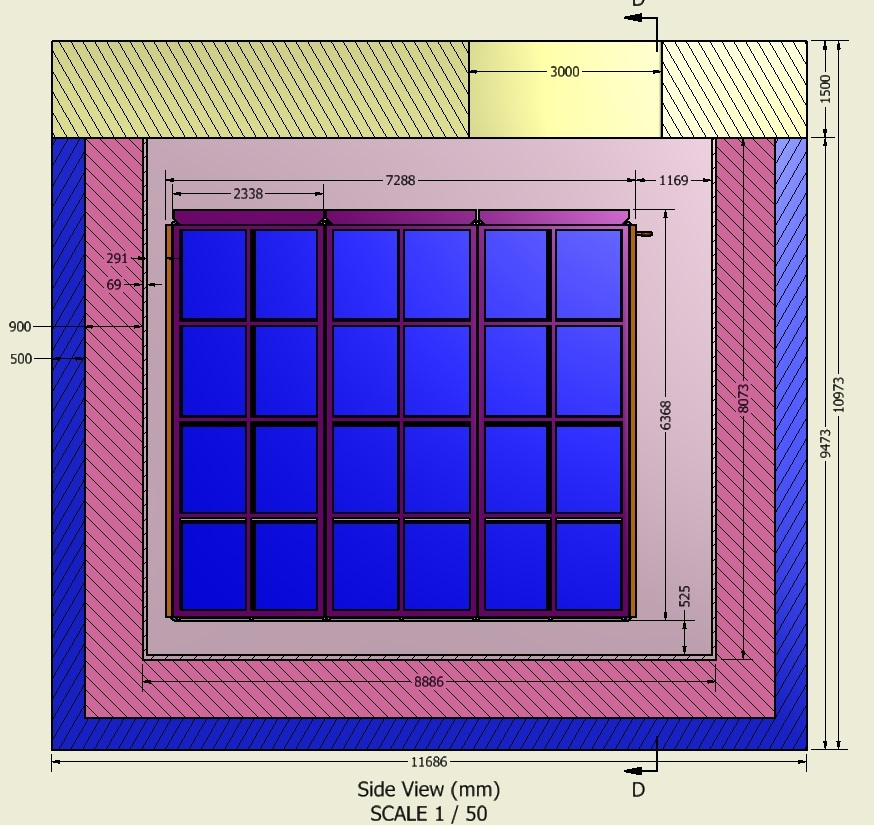
\includegraphics[width=.53\textwidth]{figures/cryostat-side-view} 
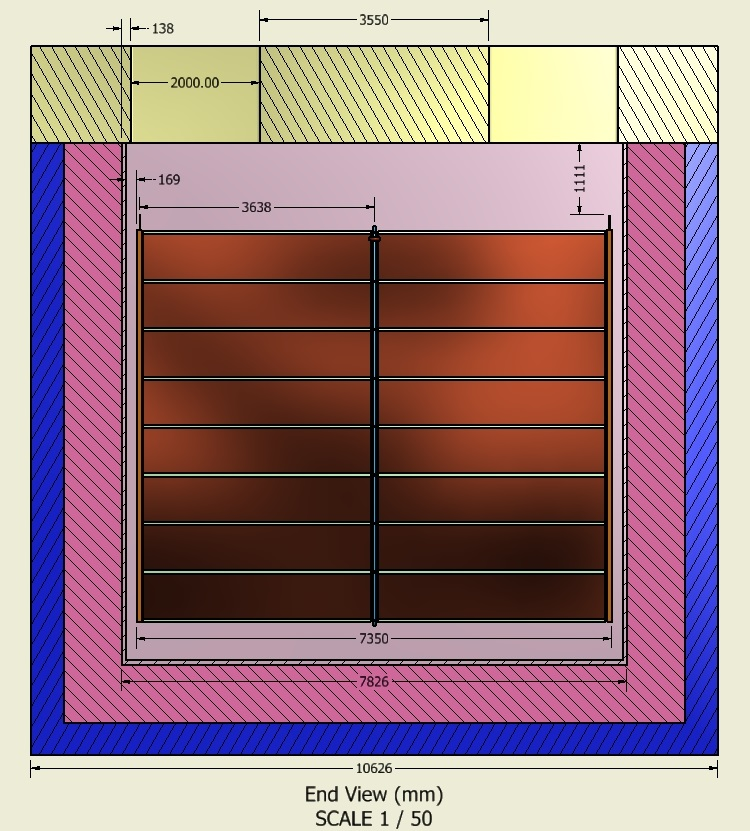
\includegraphics[width=.455\textwidth]{figures/cryostat-westend-view}  
\caption[Views of cryostat]{Side (left) and end (right) views of cryostat}
\label{fig:cryostat-views} 
\end{center}
\end{figure}
%
The beam window design is still being worked on and may lead to minor modifications if
any of the current boundaries conditions listed above is violated.
  

The cryostat has an inner volume of 483 m$^3$ and can contain  673 tons of LAr.
%
%The design is based on a scaled up version of the LBNE 35-ton Prototype\cite{montanari_35ton} 
%% (this is a comment) add \cite{montanari_sbn_perf} if public access in docdb 9270 (AH)
%and the Fermilab Short-Baseline Near Detector\cite{acciarri_sbn_proposal}.  
%
The cryostat will use a steel outer supporting structure with a metal liner inside to isolate the insulation volume, similar to the one of the dual phase WA105 detector, the $1\times1\times3$~m$^3$ prototype and to the Fermilab Short-Baseline Near Detector. 
The support structure will rest on I-beams to allow for air circulation underneath in order to maintain the temperature within the allowable limits. The proposed design encompasses the following components:
%
\begin{itemize}
\item steel outer supporting structure,
\item main body of the membrane cryostat (sides and floor), 
\item top cap of the membrane cryostat,
\item beam windows.
\end{itemize}
%
A membrane cryostat design commonly used for liquefied natural gas (LNG) storage and transportation will be used. In this vessel a stainless steel membrane contains the liquid cryogen. The pressure loading of the liquid cryogen is transmitted through rigid foam insulation to the surrounding outer support structure, which provides external support. The membrane is corrugated to provide strain relief resulting from temperature related expansion and contraction. The vessel is completed with a top cap that uses the same technology.

Two membrane cryostat vendors are known: GTT (Gaztransport \& Technigaz) from France and IHI (Ishikawajima-Harima Heavy Industries) from Japan. Each one is technically capable of delivering a membrane cryostat that meets the design requirements for this detector. To provide clarity, only one vendor is represented in this document, GTT; this is for informational purposes only. Figure~\ref{fig:lar-org} shows a 3D model of the GTT membrane and insulation design.

\begin{figure}[htbp]
\begin{center}
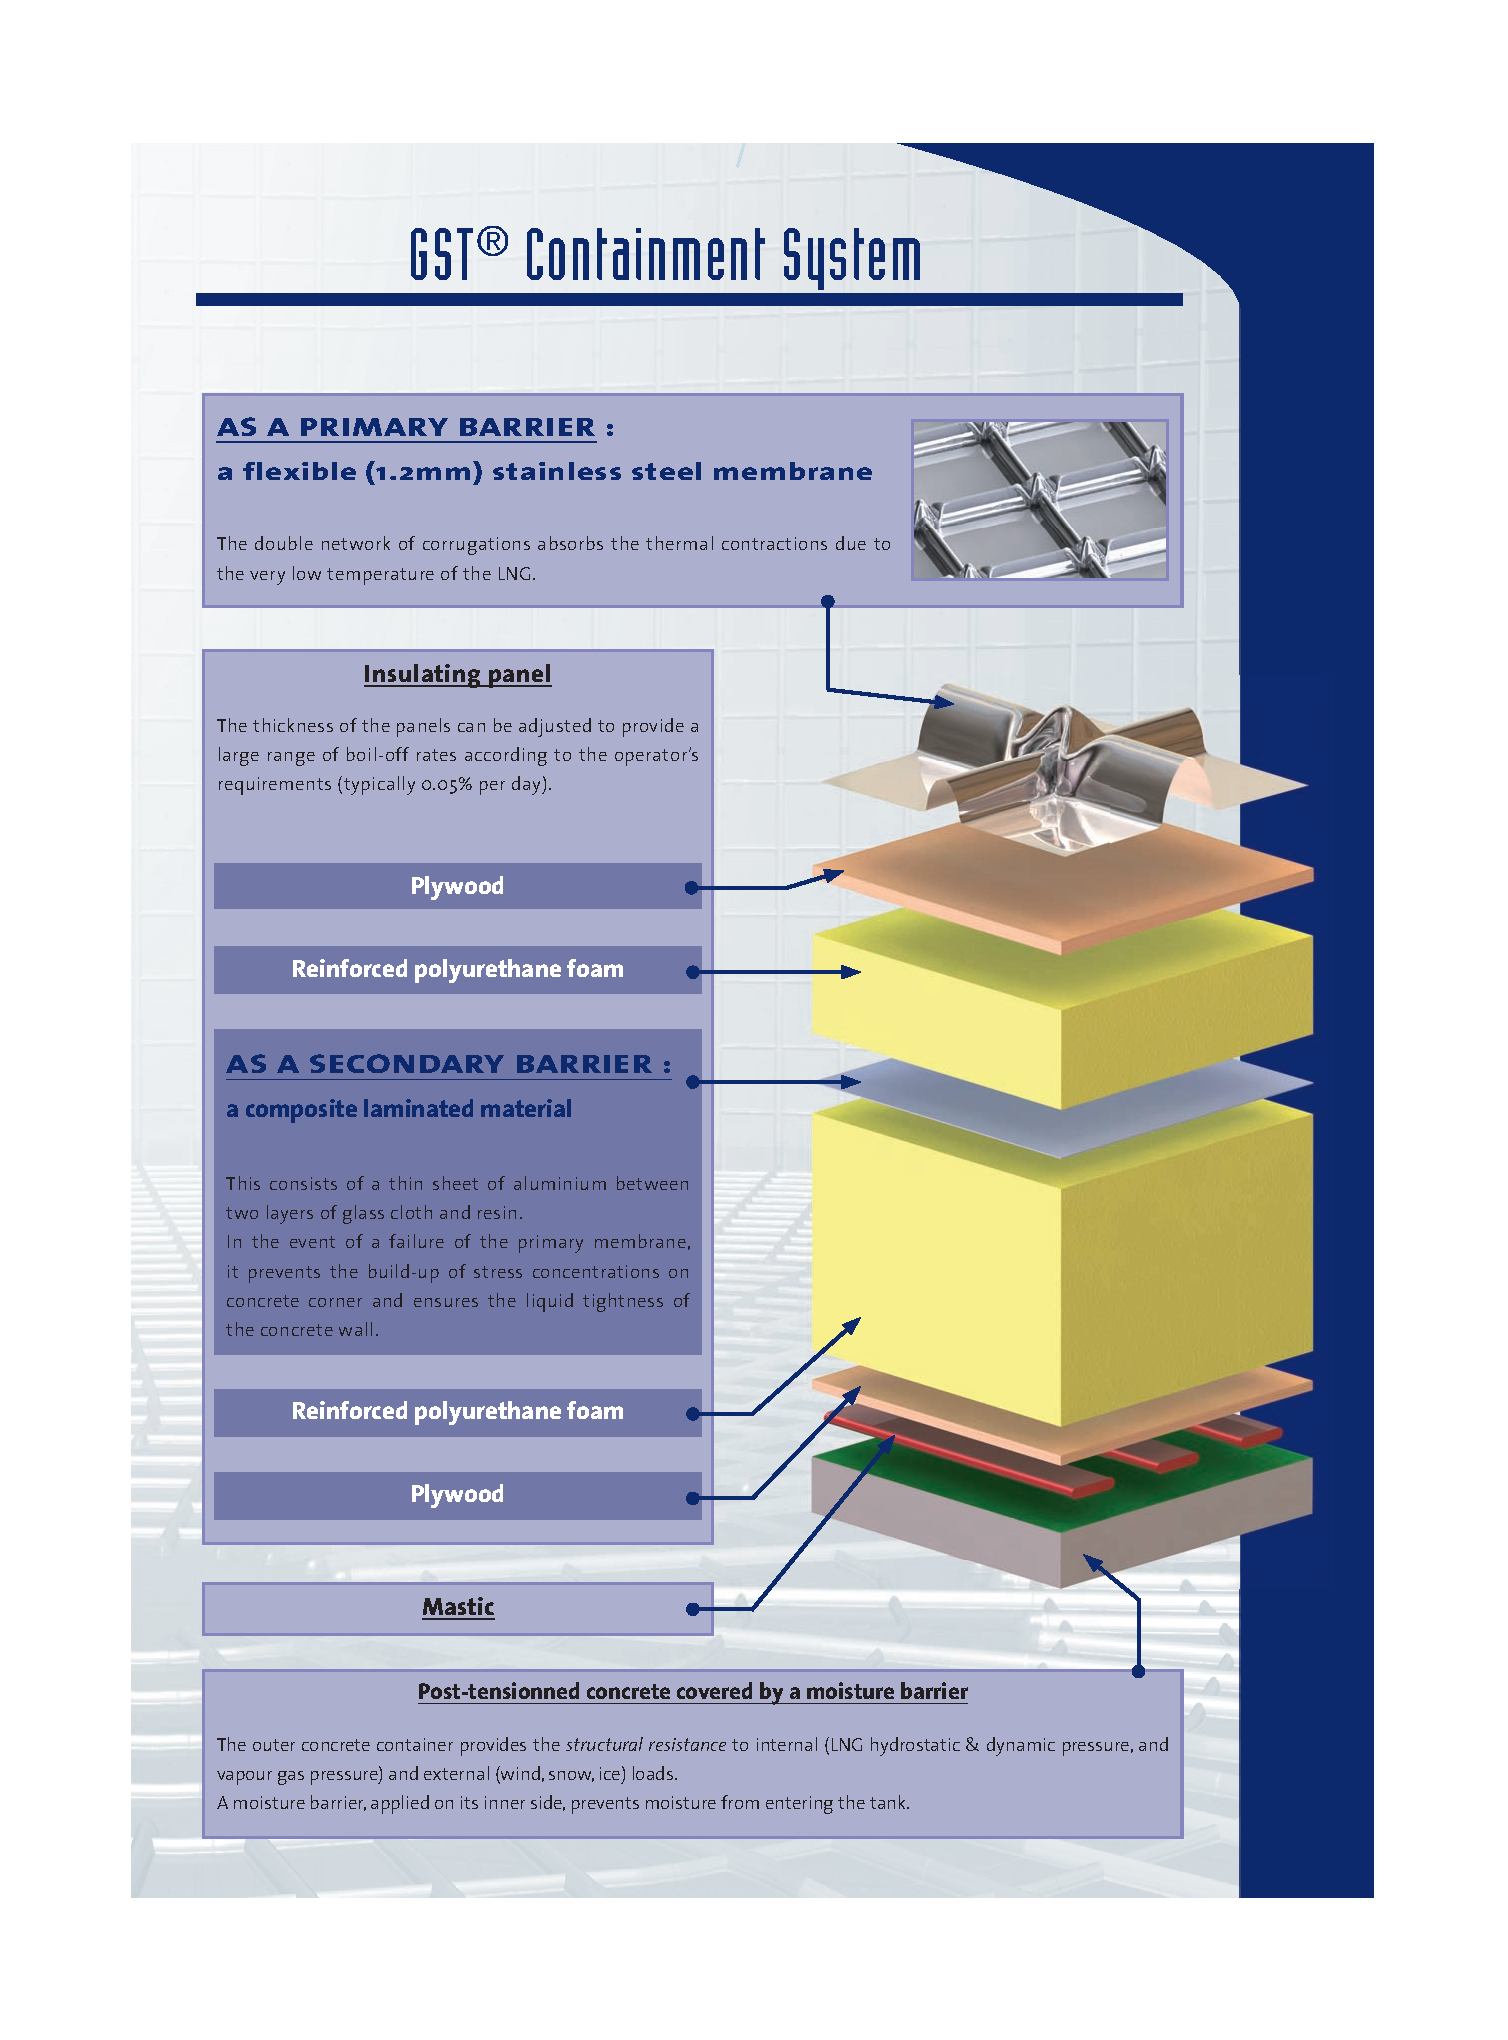
\includegraphics[width=.9\textwidth]{figures/membrane-exploded-view}
\caption[Exploded view of the membrane cryostat technology]{ Exploded view of the membrane cryostat technology}
\label{fig:lar-org}
\end{center}
\end{figure}

To minimize the contamination from warm surfaces, during operation the temperature of all surfaces in the ullage shall be lower than 100~K. 
It has been observed in the Materials Test Stand (MTS) and the Liquid Argon Purity Demonstrator (LAPD) at Fermilab that the outgassing is significantly reduced below 100~K \cite{outgassing}. A possible way to achieve this requirement is to spray a mist of clean liquid and gaseous argon to the metal surfaces in the ullage and keep them cold, similar to the strategy that was developed for the cool down of the LBNE 35 Ton prototype.

The top plate will contain two hatches for the installation of the TPCs; it will also contain a manhole to enter the tank after closing the hatches, and several penetrations for the cryogenic system and the detector. 

%\begin{figure}[htb]
%\begin{center}
%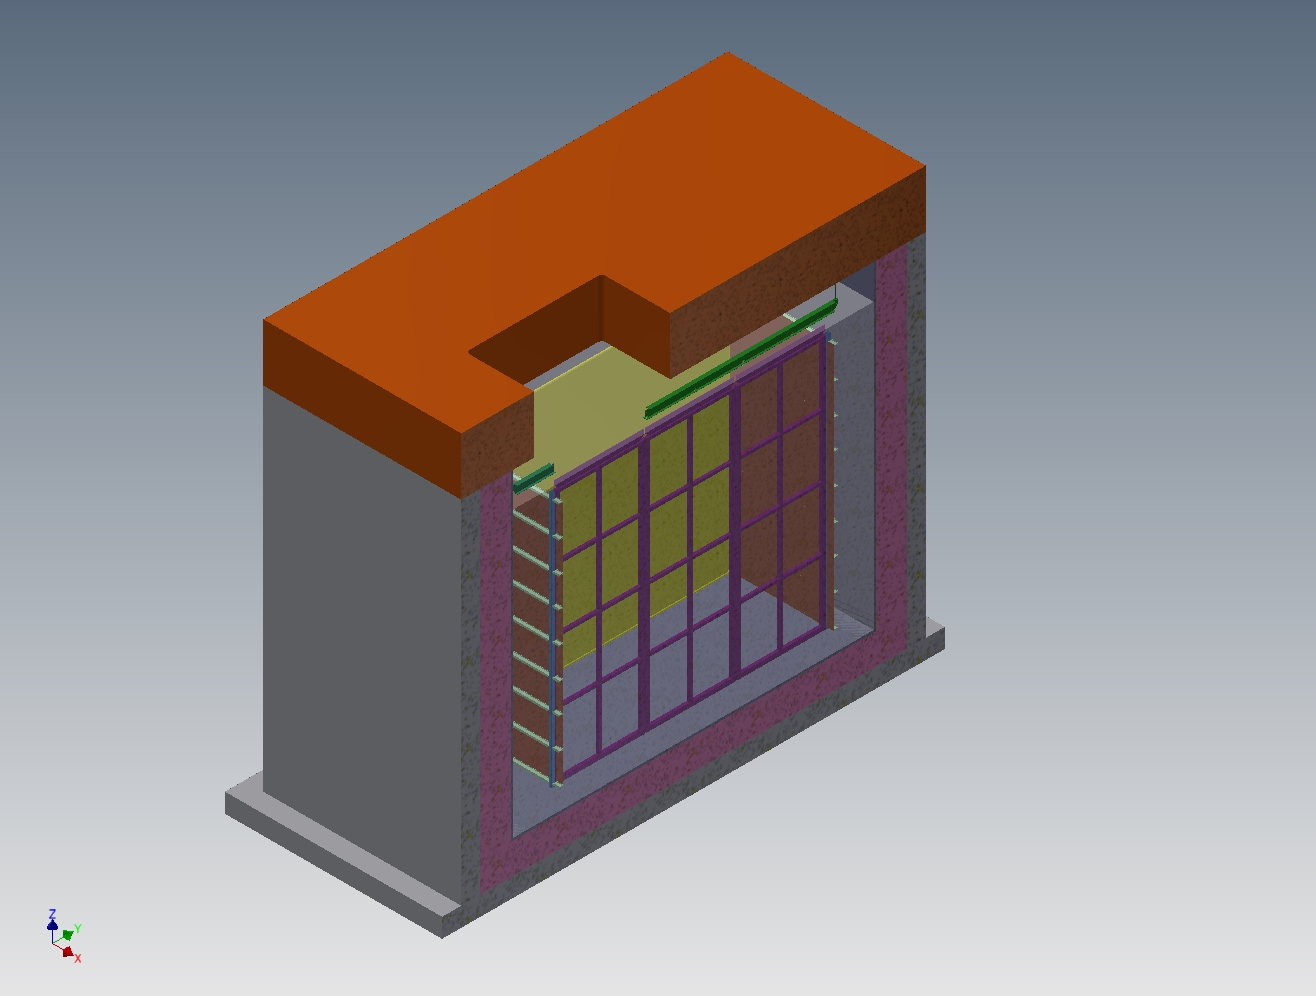
\includegraphics[width=.75\textwidth]{figures/cryostat-isometric-view} 
%\caption[Isometric view of cryostat]{\label{fig:cryostat-views} Isometric view of the membrane cryostat}
%\end{center}
%\end{figure}

%\textbf{Design Parameters:}
%
The cryostat design for the CERN prototypes includes technical solutions that are of interested for the future needs of the DUNE program. For example the use of a cold ullage (\textless  100~K) to lower the impurities in the gas region, and of a LAr pump outside the cryostat to minimize the effect of noise, vibration and microphonics to the TPC inside the liquid argon volume.
%
The design parameters for the TPC Test at CERN cryostat are listed in Table~\ref{tbl:cryogenics-design-parameters}.

\begin{table}[htpb]
\centering
\begin{tabular}{|p{.4\textwidth}|p{.5\textwidth}|}
\hline
\textbf{Design Parameter} & \textbf{Value} \\ \hline
Type of structure & Membrane cryostat \\ \hline
Membrane material    &  SS 304/304L, 316/316L or equivalent. \\ \hline
Fluid & Liquid argon (LAr)  \\ \hline
Other materials upon approval.\\ \hline
 Outside reinforcement (support structure)  &  Steel enclosure with metal liner to isolate the outside from the insulation space, standing on legs to allow for air circulation underneath. \\ \hline
 Total cryostat volume  &  538 m$^3$ \\ \hline
 Total LAr volume  &  483 m$^3$ \\ \hline
LAr total mass   & 673,000 kg  \\ \hline
Minimum inner dimensions (flat plate to flat plate).   &  7.8 m (W) x 8.9 m (L) x 8.1 0 (H) \\ \hline
Depth of LAr   &  7.2 m (0.82 m ullage, same as LBNF) \\ \hline
Primary membrane   &   1.2 mm thick SS 304L corrugated stainless steel\\ \hline
Secondary barrier system   &  GTT design; 0.07 mm thick aluminum between fiberglass cloth. Overall thickness 1 mm located between insulation layers.  \\ \hline
 Insulation  &  Polyurethane foam (0.9 m thick from preliminary calculations) \\ \hline
Maximum static heat leak   &  10 W/m$^2$ \\ \hline
LAr temperature   & 88 +/- 1K  \\ \hline
Operating gas pressure   &  Positive pressure. Nominally 70 mbarg ($\sim$1 psig) \\ \hline
 Vaccuum  &  No vacuum \\ \hline
 Design pressure  &  350 mbarg ($\sim$5 psig) + LAr head (1,025 mbarg) \\ \hline
Design temperature   &  77 K (liquid nitrogen temperature for flexibility) \\ \hline
Temperature of all surfaces in the ullage during operation   & \textless 100 K  \\ \hline
Leak tightness   & $10^{-6}$ mbar*l/sec   \\ \hline
Maximum noise/vibration/microphonics inside the cryostat   & LAr pump outside the cryostat  \\ \hline
Beam window   & Precise location TBD. Multiple beam windows installed on the upstream side of the cryostat  \\ \hline
 Accessibility after operations  & Capability to empty the cryostat in 30 days and access it in 60 days after the end of operations. \\ \hline
  Lifetime / Thermal cycles &  Consistent with liquid argon program. TBD. \\ \hline
 \end{tabular}
\caption{Design requirements for the membrane cryostat}
\label{tbl:cryogenics-design-parameters}
\end{table}

\textbf{Insulation system and secondary membrane: }
%
The membrane cryostat requires insulation applied to all internal surfaces of the outer support structure 
and roof in order to control the heat ingress and hence required refrigeration heat load. 
To avoid bubbling of the liquid argon inside the tank, the maximum static heat leak is 10 W/m$^2$ for the floor and the sides and 15 W/m$^2$ for the roof, higher to account for the penetrations that increase the heat budget. Preliminary calculations show that these values can be obtained using 0.9 m thick insulation panels of polyurethane foam.
Given an 
average thermal conductivity coefficient for the insulation material of 0.0283 W/(m$\cdot$K), the heat input 
from the surrounding steel is expected to be about 3.2~kW total. It assumes that the hatches are foam 
insulated as well. This is shown in Table~\ref{tbl:heat-load-calc}.

The insulation material is a solid reinforced polyurethane foam manufactured as composite panels. The 
panels get laid out in a grid with 3 cm gaps between them (that will be filled with fiberglass) and fixed 
onto anchor bolts anchored to the support structure. The composite panels contain the two layers of 
insulation with the secondary barrier in between. After positioning adjacent composite panels and filling 
the 3-cm gap, the secondary membrane is spliced together by epoxying an additional overlapping layer 
of secondary membrane over the joint. All seams are covered so that the secondary membrane is a 
continuous liner.

In the GTT design, the secondary membrane is comprised of a thin aluminum sheet and 
fiberglass cloth. The fiberglass-aluminum-fiberglass composite is very durable and flexible with an 
overall thickness of about 1 mm. The secondary membrane is placed within the insulation space. It 
surrounds the bottom and sides. In the unlikely event of an internal leak from the primary membrane of 
the cryostat into the insulation space, it will prevent the liquid cryogen from migrating all the way 
through to the steel support structure where it would degrade the insulation thermal performance and 
could possibly cause excessive thermal stress in the support structure. The liquid cryogen, in case of 
leakage through the inner (primary) membrane will escape to the insulation volume, which is purged with 
GAr at the rate of one volume exchange per day.

\begin{table}[htpb]
\centering
\begin{tabular}{|p{.15\textwidth}|p{.15\textwidth}|p{.15\textwidth}|p{.15\textwidth}|p{.15\textwidth}|}
\hline
 \textbf{Element} & \textbf{Area ($m^2$)}  &  \textbf{K ($W/mK$)} & \textbf{$\Delta$ T ($K$)}
 & \textbf{Heat Input ($W$)}\\ \hline
Base   & 83  & 0.0283   &205   & 534 \\ \hline
End walls  &  153 & 0.0283  &  205 &  986 \\ \hline
Side walls   & 172  & 0.0283  &  205 & 1,108 \\ \hline
Roof  &  83 & 0.0283  & 205  &  550\\ \hline
   &   &   &   &  \\ \hline
Total   &   &   &   & 3,162 \\ \hline
\end{tabular}
\caption{Heat load calculation for the membrane cryostat (insulation thickness=0.9~m). }
\label{tbl:heat-load-calc}
\end{table}


\textbf{Outer Support Structure:}
%
The proposed design is a steel support structure with a metal liner on the inside to isolate the insulation region and keep the moisture out. This choice allows natural and forced ventilation to maintain the temperature of the steel within its limit, without the need of heating elements and temperature sensors. 
The main body of the membrane cryostat does not have side openings for construction. The access is only from the top. There is a side penetration for the liquid argon pump for the purification of the cryogen.

%\textbf{Main body of the membrane cryostat:}
%
%The sides and bottom of the vessel constitute the main body of the membrane cryostat. They consist of several layers. From the inside to the outside the layers are stainless steel primary membrane, insulation, thin aluminum secondary membrane, more insulation, and steel outer support structure with meal panels acting as vapor barier. The secondary membrane contains the LAr in case of any primary membrane leaks and the vapor barrier prevents water ingress into the insulation. 


\textbf{Top cap:}
%
Several steel reinforced plates welded together constitute the top cap. The stainless steel primary 
membrane, intermediate insulation layers and vapor barrier continue across the top of the detector, 
providing a leak tight seal. The secondary barrier is not used nor required at the top. The cryostat roof is 
a removable steel truss structure that also supports the detector. Stiffened steel plates are welded to the 
underside of the truss to form a flat vapor barrier surface onto which the roof insulation attaches directly. 
The penetrations will be clustered in one region. The top cap will have two large openings for TPC 
installation, and a manhole to enter the tank  after the 
hatches have been closed.

The truss structure rests on top of the supporting structure where a positive structural connection 
between the two is made to resist the upward force caused by the slightly pressurized argon in the ullage 
space. The hydrostatic load of the LAr in the cryostat is carried by the floor and the sidewalls. In order to meet the maximum deflection of 3~mm between APA and CPA 
and to decouple the detector from possible sources of vibrations, the TPCs will be connected to an external bridge over the top of the plate supported on the floor of the building. Everything else within the cryostat %(TPC planes, 
(electronics, sensors, cryogenic and gas plumbing connections) is 
supported by the steel plates under the truss structure. All piping and electrical penetration into the 
interior of the cryostat are made through this top plate, primarily in the region of the penetrations to 
minimize the potential for leaks. Studs are welded to the underside of the top plate to bolt the insulation 
panels. Insulation plugs are inserted into the bolt-access holes after panels are mounted. The primary 
membrane panels are first tack-welded then fully welded to complete the inner cryostat volume.
%
Table~\ref{tbl:cryostat-top-parameters} presents the list of the design parameters for the top of the cryostat.
%
\begin{table}[htpb]
\centering
\begin{tabular}{|p{.3\textwidth}|p{.7\textwidth}|} % AH {|p{.4\textwidth}|p{.5\textwidth}|}
\hline
 \textbf{Design Parameter} & \textbf{Value} \\ \hline
 Configuration &  Removable metal plate reinforced with trusses/I-beams anchored to the membrane cryostat support structure. Contains multiple penetrations of various sizes and a manhole. Number, location and size of the penetrations TBD. The hatches shall be designed to be removable. If welded, provisions shall be made to allow for removal and re-welding six (6) times.\\ \hline
Plate/Trusses non-wet material  &  Steel if room temperature.
SS 304/304 or equivalent if at cryogenic temperature
\\ \hline
Wet material  & SS 304/304L, 316/316L or equivalent. 
Other materials upon approval.
 \\ \hline
 Fluid & Liquid argon (LAr) \\ \hline
Design pressure  & 350 mbarg (~5 psig) \\ \hline
Design temperature  & 77 K (liquid nitrogen temperature for flexibility) \\ \hline
Inner dimensions  & To match the cryostat \\ \hline
Maximum allowable roof deflection  & 0.003 m (differential between APA and CPA) \\ \hline
Maximum static heat leak  & \textless 15 W/m$^2$  \\ \hline
 Temperatures of all surfaces in the ullage during operation & \textless 100 K \\ \hline
Additional design loads  &  -	Top self-weight \\
 & -	Live load (488 kg/m$^2$)\\
& -	Electronics racks (400 kg in the vicinity of the feed through)\\
& -	Services (150 kg on every feed through)
\\ \hline
TPC anchors  & %Capacity: AH
Number and location TBD. Minimum 6.
 \\ \hline
 Hatch opening for TPCs installation &  3.550 m x 2.000 m (location TBD)\\ \hline % , to . in numbers
Grounding plate  &  1.6 mm thick copper sheet brazed to the bottom of the top plate\\ \hline
Lifting fixtures  & Appropriate for positioning the top at the different parts that constitute it. \\ \hline
Penetrations  &  1 LAr In, 1 Purge GAr In, 1 Vent GAr In \\ 
& 2 Pressure Safety Valves, 2 Vacuum Safety Valves \\ 
& 1 GAr boil off to condenser \\ 
& 1-2 Liquid level sensors \\ 
& 1-2 Instrumentation \\ 
& 1 Temperature sensors feedthroughs? \\ 
& 1 LAr for cool down, 1 GAr for cool down \\ 
& 1 TPC signal, 3 TPC feedthroughs \\
& 1 Photon Detector for APA (Cold) \\
& Calibration dc\\ \hline
Lifetime / Thermal cycles  & Consistent with the liquid argon program TBD. \\ \hline
\end{tabular}
\caption{Design parameters for the top of the cryostat}
\label{tbl:cryostat-top-parameters}
\end{table}

\textbf{Beam windows:}
%%%%%%%%%%%%%%%%%%%%%%%%%%%%%%%%%%%%%%%%%%%%%%%%%%%%
%Discussion on preliminary beam window design ( C. Lin)
%%%%%%%%%%%%%%%%%%%%%%%%%%%%%%%%%%%%%%%%%%%%%%%%%%%%
Multiple beam windows will be installed along the horizontal midplane
on the upstream side of the LAr cryostat to allow particle beam to
enter the active TPC volume with minimal energy loss and scattering.
To simplify the mechanical design, we are exploring installing
multiple modular beam windows as opposed to a single monolithic beam
window. Each beam window will be identical in design and has a nominal
circular cross section of about 20 cm in diameter. The window will be
installed into a frame. The frame is assembled into the cryostat wall
by the vendor at time of fabrication, and includes seals to both
primary and secondary membranes. Inside the LAr volume, there will be low
density "plugs" to displace the passive volume of LAr along the beam
path length before the active TPC volume. The window design and
configuration have not been finalized. There will likely be three or
more beam windows installed on the cryostat to allow the beam to enter
the cryostat at different locations and angles. Windows not being used
for the active beam configuration will be covered by exterior flanges
for safety.
%%%%%%%%%%%%%%%%%%%%%%%%%%%%%%%%%%%%%%%%%%%%%%%%%%%%

\textbf{Cryostat grounding and isolation requirements:}
%
The cryostat has to be grounded and electrically isolated from the building. 
Figure~\ref{fig:top-plate-gnd} shows the layout of the top plate grounding.
We list the grounding and isolation requirements for the cryostat. 

\begin{enumerate}
\item \textbf{Isolation}
	\begin{enumerate}
	\item The cryostat membrane and any supporting structure, whether it is a steel structure or a concrete and rebar pour, shall be isolated from any building metal or building rebar with a DC impedance greater than 300 k$\Omega$.
	\item All conductive piping penetrations through the cryostat shall have dielectric breaks prior to entering the cryostat and the top plate.
	\end{enumerate}

\item \textbf{Grounding}
	\begin{enumerate}
	\item The cryostat, or ``detector'' ground, shall be separated from the ``building'' ground.
	\item A safety ground network consisting of saturated inductors shall be used between detector ground and building ground.
	\end{enumerate}

\item \textbf{Top plate grounding}
	\begin{enumerate}
	\item The top grounding plate shall be electrically connected to the cryostat membrane by means of copper braid connections.
	   \begin{enumerate}
	   \item Each connection shall be at least 1.6 mm thick and 63.5 mm wide.
	   \item The length of each connection is required to be as short as possible.
	   \item The distance between one connection and the next one shall be no more than 1.25 m.
	   \item The layout can follow the profile of several pieces of insulation, but it shall be continuous.	
	   \item The DC impedance of the membrane to the top plate shall be less than 1 ohm.
	   \end{enumerate}
	\end{enumerate}
\end{enumerate}


\begin{figure}
\begin{center}
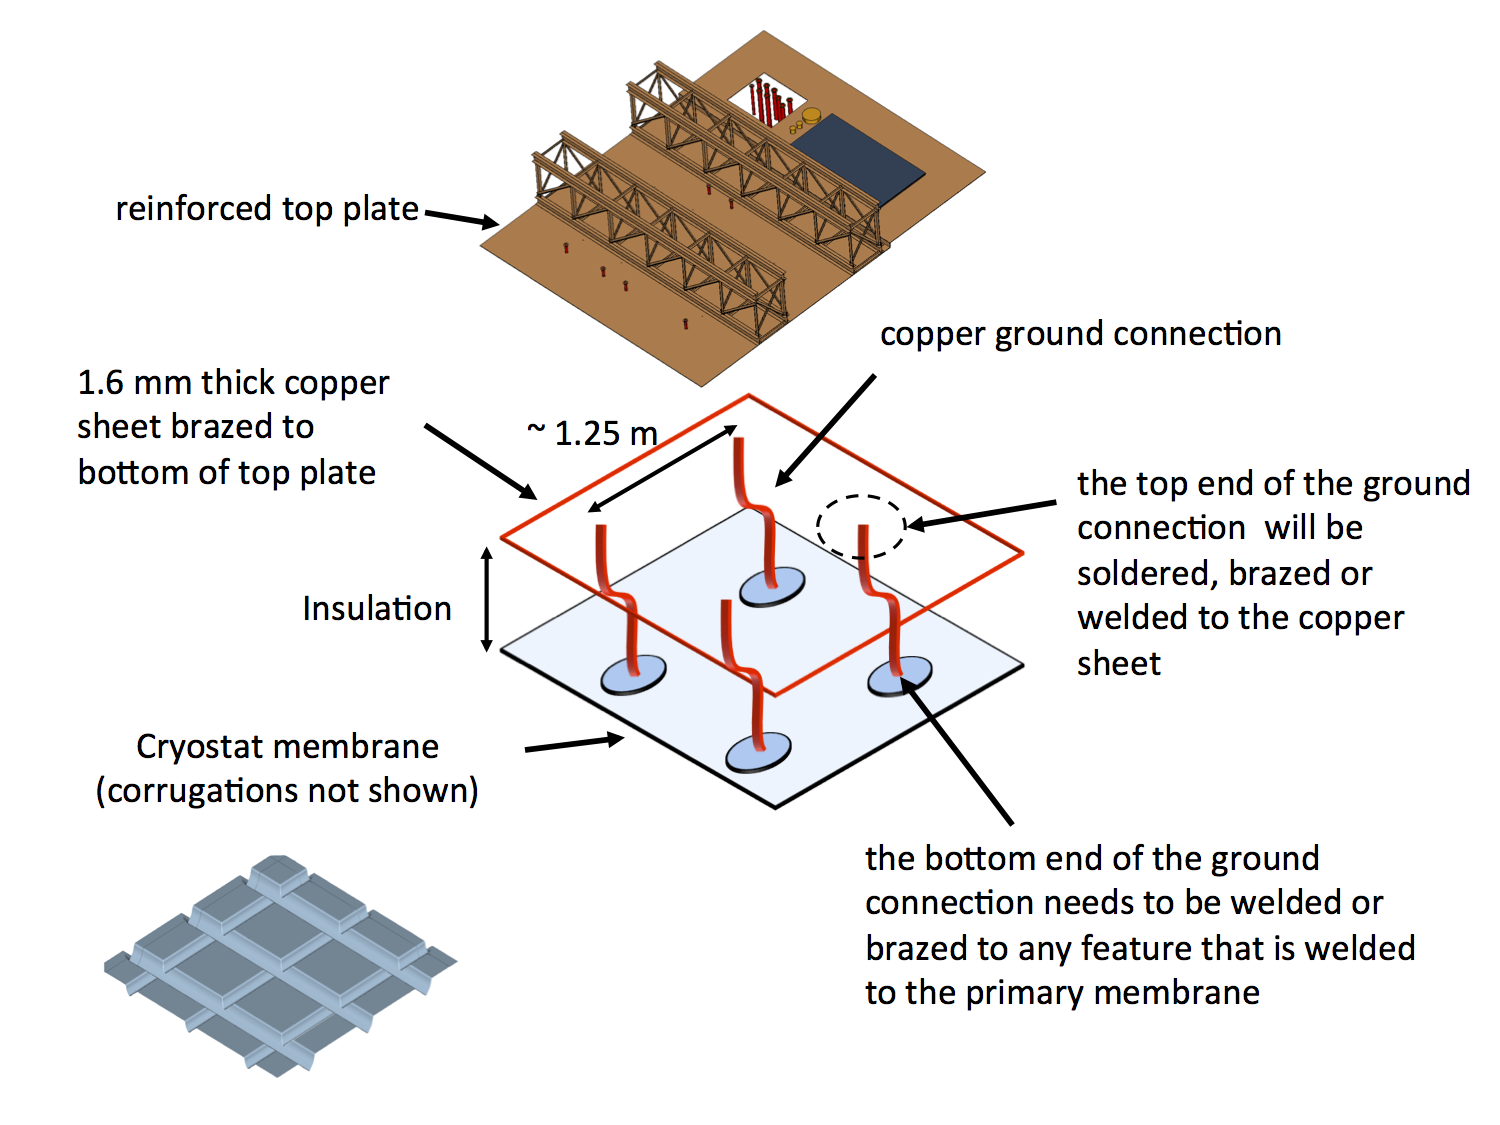
\includegraphics[width=1.0\textwidth]{figures/cryostat-top-plate-gnd} 
\caption[Top plate grounding layout]{\label{fig:top-plate-gnd}Top plate grounding layout}
\end{center}
\end{figure}

\textbf{Leakage quality assurance: }
%
The primary membrane will be subjected to several leak tests and weld remediation, as necessary. All 
(100\%) of the welds will be tested by an Ammonia colorimetric leak test (ASTM E1066-95) in which 
welds are painted with a reactive yellow paint before injecting a Nitrogen-Ammonia mixture into the 
insulation space of the tank. Wherever the paint turns purple or blue, a leak is present. The developer is 
removed, the weld fixed and the test is performed another time. Any and all leaks will be repaired. The 
test lasts a minimum of 20 hours and is sensitive enough to detect defects down to 0.003 mm in size 
and to a 10$^{-7}$ std-cm$^3/s$ leak rate (equivalent leak rate at standard pressure and temperature, 1 bar and 
273 K). To prevent infiltration of water vapor or oxygen through microscopic membrane leaks (below 
detection level) the insulation spaces will be continuously purged with gaseous argon to provide one 
volume exchange per day. The insulation space will be maintained at 70 mbar, slightly above 
atmospheric pressure. This space will be monitored for changes that might indicate a leak from the 
primary membrane. Pressure control devices and safety relief valves will be installed on the insulation 
space to ensure that the pressure does not exceed the operating pressure inside the tank. The purge gas 
will be recirculated by a blower, purified, and reused as purge gas. The purge system is not safety-
critical; an outage of the purge blower would have negligible impact on LAr purity.


%%%%%%%%%%%%%%%%%
\subsection{Cryogenic System}

Figure~\ref{fig:proposed-LN2-system} outlines the basic scheme of the LN2 supply system, which was 
proposed by CERN for the Short Baseline Program and found to be an appropriate solution for this 
detector as well. 
%
\begin{figure}[htb]
\begin{center}
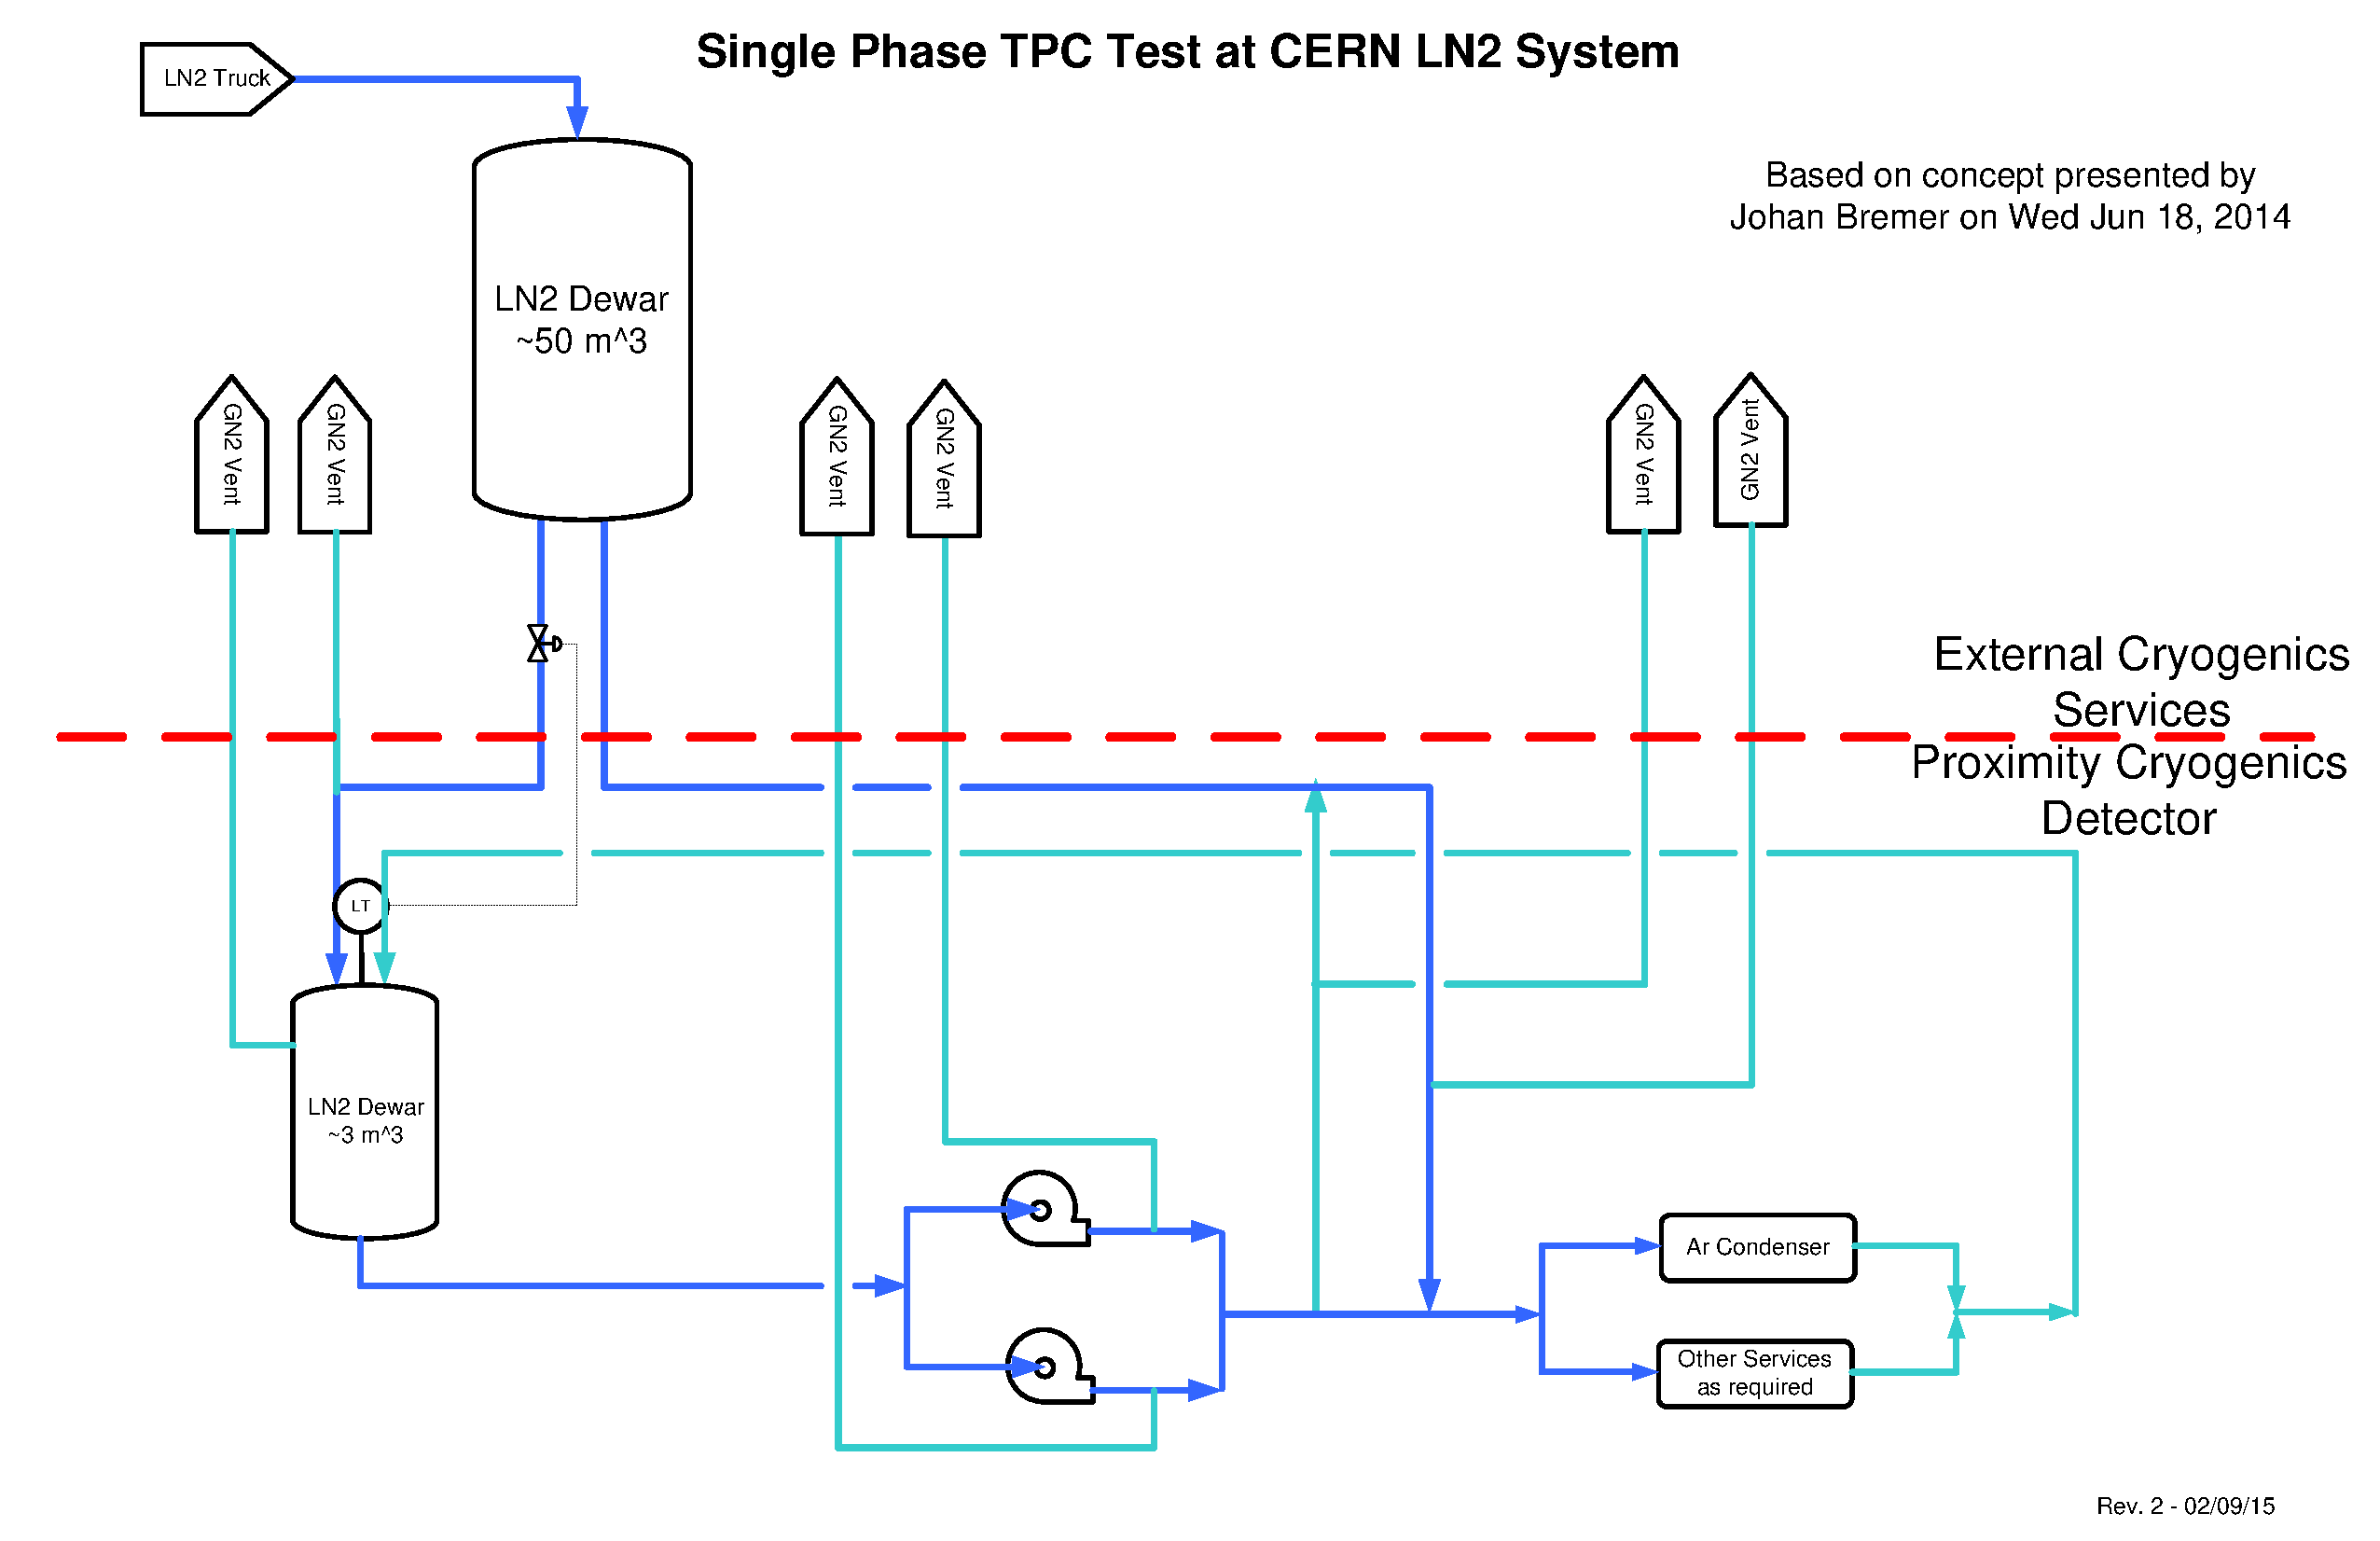
\includegraphics[width=.95\textwidth]{figures/proposed-LN2-system} 
\caption[Schematic diagram for the proposed LN2 system.]{\label{fig:proposed-LN2-system}Schematic diagram for the proposed LN2 system}
\end{center}
\end{figure}
%
The experiment will rely on LN2 tankers for regular deliveries to a local dewar storage, 
which will be sized to provide several days of cooling capacity in the event of a delivery interruption. 
From the dewar storage the LN2 is then transferred to a distribution facility located in the experimental 
hall. It includes a small buffer volume and an LN2 pumping station that transfers the LN2 to the argon 
condenser and other services as needed. The low estimated heat leak of the vessel ($\sim$3.2~kW) and the 
location inside an above ground building allow for use of an open loop system typical of other 
installations operated at Fermilab (LAPD, LBNE 35 ton prototype, MicroBooNE) and at CERN. 
The main goal of the LN2 system is to provide cooling power for the argon condenser, the initial cool down of 
the vessel and the detector, and all other services as needed.
%
 Table~\ref{tbl:cryo-design-parameters} presents the list of 
requirements for the cryogenic system for the single phase detector test at CERN.
%
\begin{table}[htbp]
\centering
\begin{tabular}{|p{.45\textwidth}|p{.45\textwidth}|}
\hline
 \textbf{ Parameter} & \textbf{Value} \\ \hline
 Location & Preferably not in front of the cryostat (on the beam) \\ \hline
 Cooling Power & TBD based on the heat leak of the cryostat (estimated 3.4~kW), the cryo-piping and all other contributions (cryogenic pumps, etc.) \\ \hline
 Liquid argon purity in cryostat & 10 ms electron lifetime (30 ppt O2 equivalent) \\  \hline
 Gaseous argon piston purge rate of rise & 1.2 m/hr \\ \hline
 Membrane cool-down rate & From manufacturer \\  \hline
 TPCs cool-down rate & \textless40 K/hr,\textless10 K/m (vertically)
 \\ \hline
Mechanical load on TPC & The LAr or the gas pressure shall not apply a mechanical load to the TPC greater than 200 Pascal. \\ \hline
Nominal LAr purification flow rate (filling/ops) & 5.5 day/volume exchange \\ \hline
 Temperature of all surfaces in the ullage during operations & \textless100 K \\  \hline
 Gaseous argon purge within insulation & 1 volume change /day of the open space between insulation panels. \\ \hline
 Lifetime of the cryogenic system & Consistent with the LAr program. TBD. \\ \hline
\end{tabular}
\caption{Design requirements for the cryogenic system}
\label{tbl:cryo-design-parameters}
\end{table}
%


Figure~\ref{fig:proposed-LAr-system} shows a schematic diagram of the proposed liquid argon system. It is based on the design of the 
LBNE 35 ton prototype, the MicroBooNE detector systems and the plans for the DUNE Far Detector.
\begin{figure}
\begin{center}
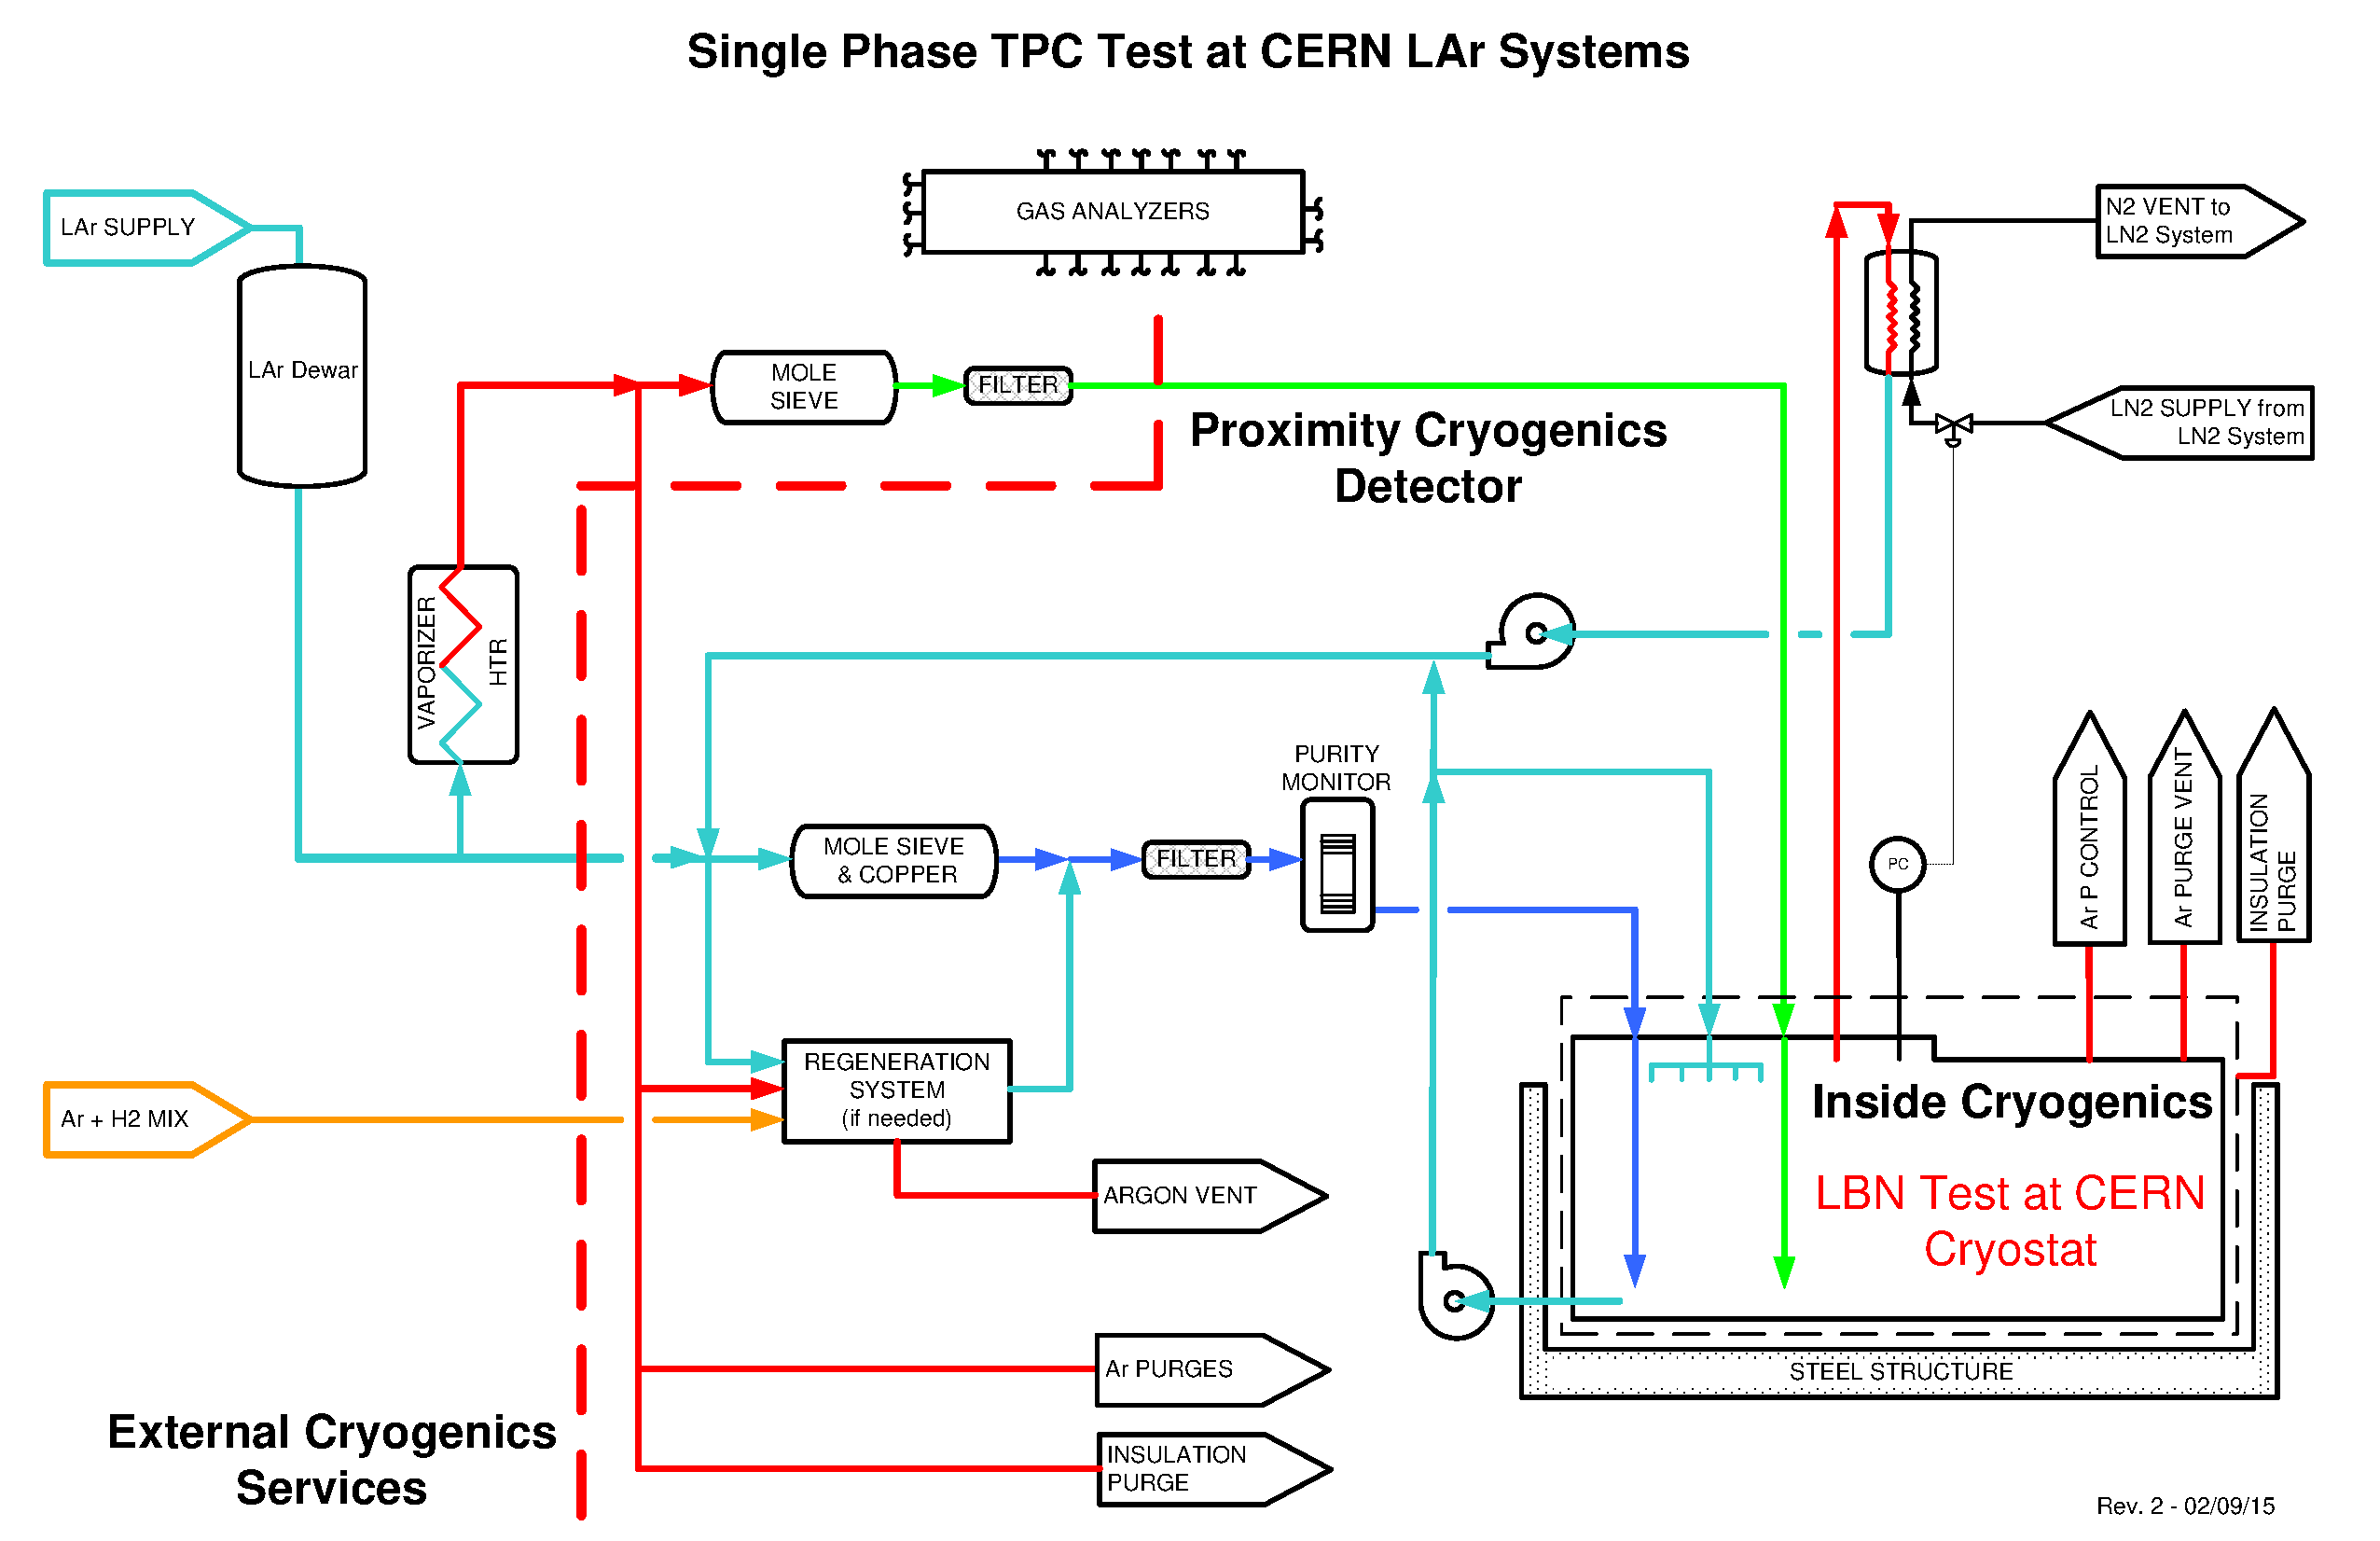
\includegraphics[width=1.0\textwidth]{figures/proposed-LAr-system} 
\caption[Schematic diagram for the proposed LAr system]{\label{fig:proposed-LAr-system} Schematic diagram for the proposed LAr system}
\end{center}
\end{figure}
The main goal of the LAr system is to purge the cryostat prior to the start of the operations (with GAr in open 
and closed loop), cool down the cryostat and fill it with LAr. Then continuously purify the LAr and the boil 
off GAr to maintain the required purity which is measured by the detector in the form of an electron drift time measurement.

The LAr receiving facility includes a storage dewar and an ambient vaporizer to deliver LAr and GAr to the 
cryostat. The LAr goes through the liquid argon handling and purification system, whereas the GAr 
through the gaseous argon purification before entering the vessel.

The LAr purification system is currently equipped with a filter containing mol sieve and copper beads, and 
a regeneration loop to regenerate the filter itself. Filters containing Oxysorb and Hydrosorb rather than 
mol sieve and copper beads represent a proven alternate solutions.
Studies are ongoing to standardize the filtration scheme and select the optimal filter medium for all 
future generation detectors, including the CERN prototypes. 

During operation, an external LAr pump circulates the bulk of the cryogen through the LAr purification 
system. The boil off gas is first recondensed and then is sent to the LAr purification system before 
re-entering the vessel.




